%!TEX program = xelatex

\documentclass{beamer}
\usetheme{metropolis}

\setbeamercolor{background canvas}{bg = white}

\usepackage{appendixnumberbeamer}
\renewcommand\appendixname{Appendix}

% packages
\usepackage{amssymb}
\usepackage{amsmath}
\usepackage{mathtools}
\usepackage{hyperref}
\usepackage{lmodern}

% graphics
\graphicspath{ {Figures/} }

\title{Queues with a Dynamic Schedule}
\author{John Gilbertson}
\date{October 2016}

\begin{document}

\begin{frame}
	\titlepage
\end{frame}

\begin{frame}
	\frametitle{Outline}
	\tableofcontents
\end{frame}

\section{Section 1}

\begin{frame}
	\frametitle{Title}
	Lorem ipsum dolor sit amet, consectetur adipisicing elit, sed do eiusmod tempor incididunt ut labore et dolore magna aliqua.

	\begin{equation}
		10 + x = y
	\end{equation}
\end{frame}

\begin{frame}
	\frametitle{List}
	\begin{itemize}
		\item Point A
		\item Point B
		\begin{itemize}
			\item Part 1
			\item Part 2
		\end{itemize}
		\item Point C
		\item Point D
	\end{itemize}
\end{frame}

\begin{frame}
	\frametitle{Using Columns}
	\begin{columns}
		\column{0.5\textwidth}
		Point 1
		\column{0.5\textwidth}
		Point 2
	\end{columns}
\end{frame}

\begin{frame}
	\frametitle{Picture}
	\begin{columns}
		\column{0.5\textwidth}
		\begin{itemize}
			\item<2-> Description
		\end{itemize}
		\column{0.5\textwidth}
		\begin{figure}
			\centering
			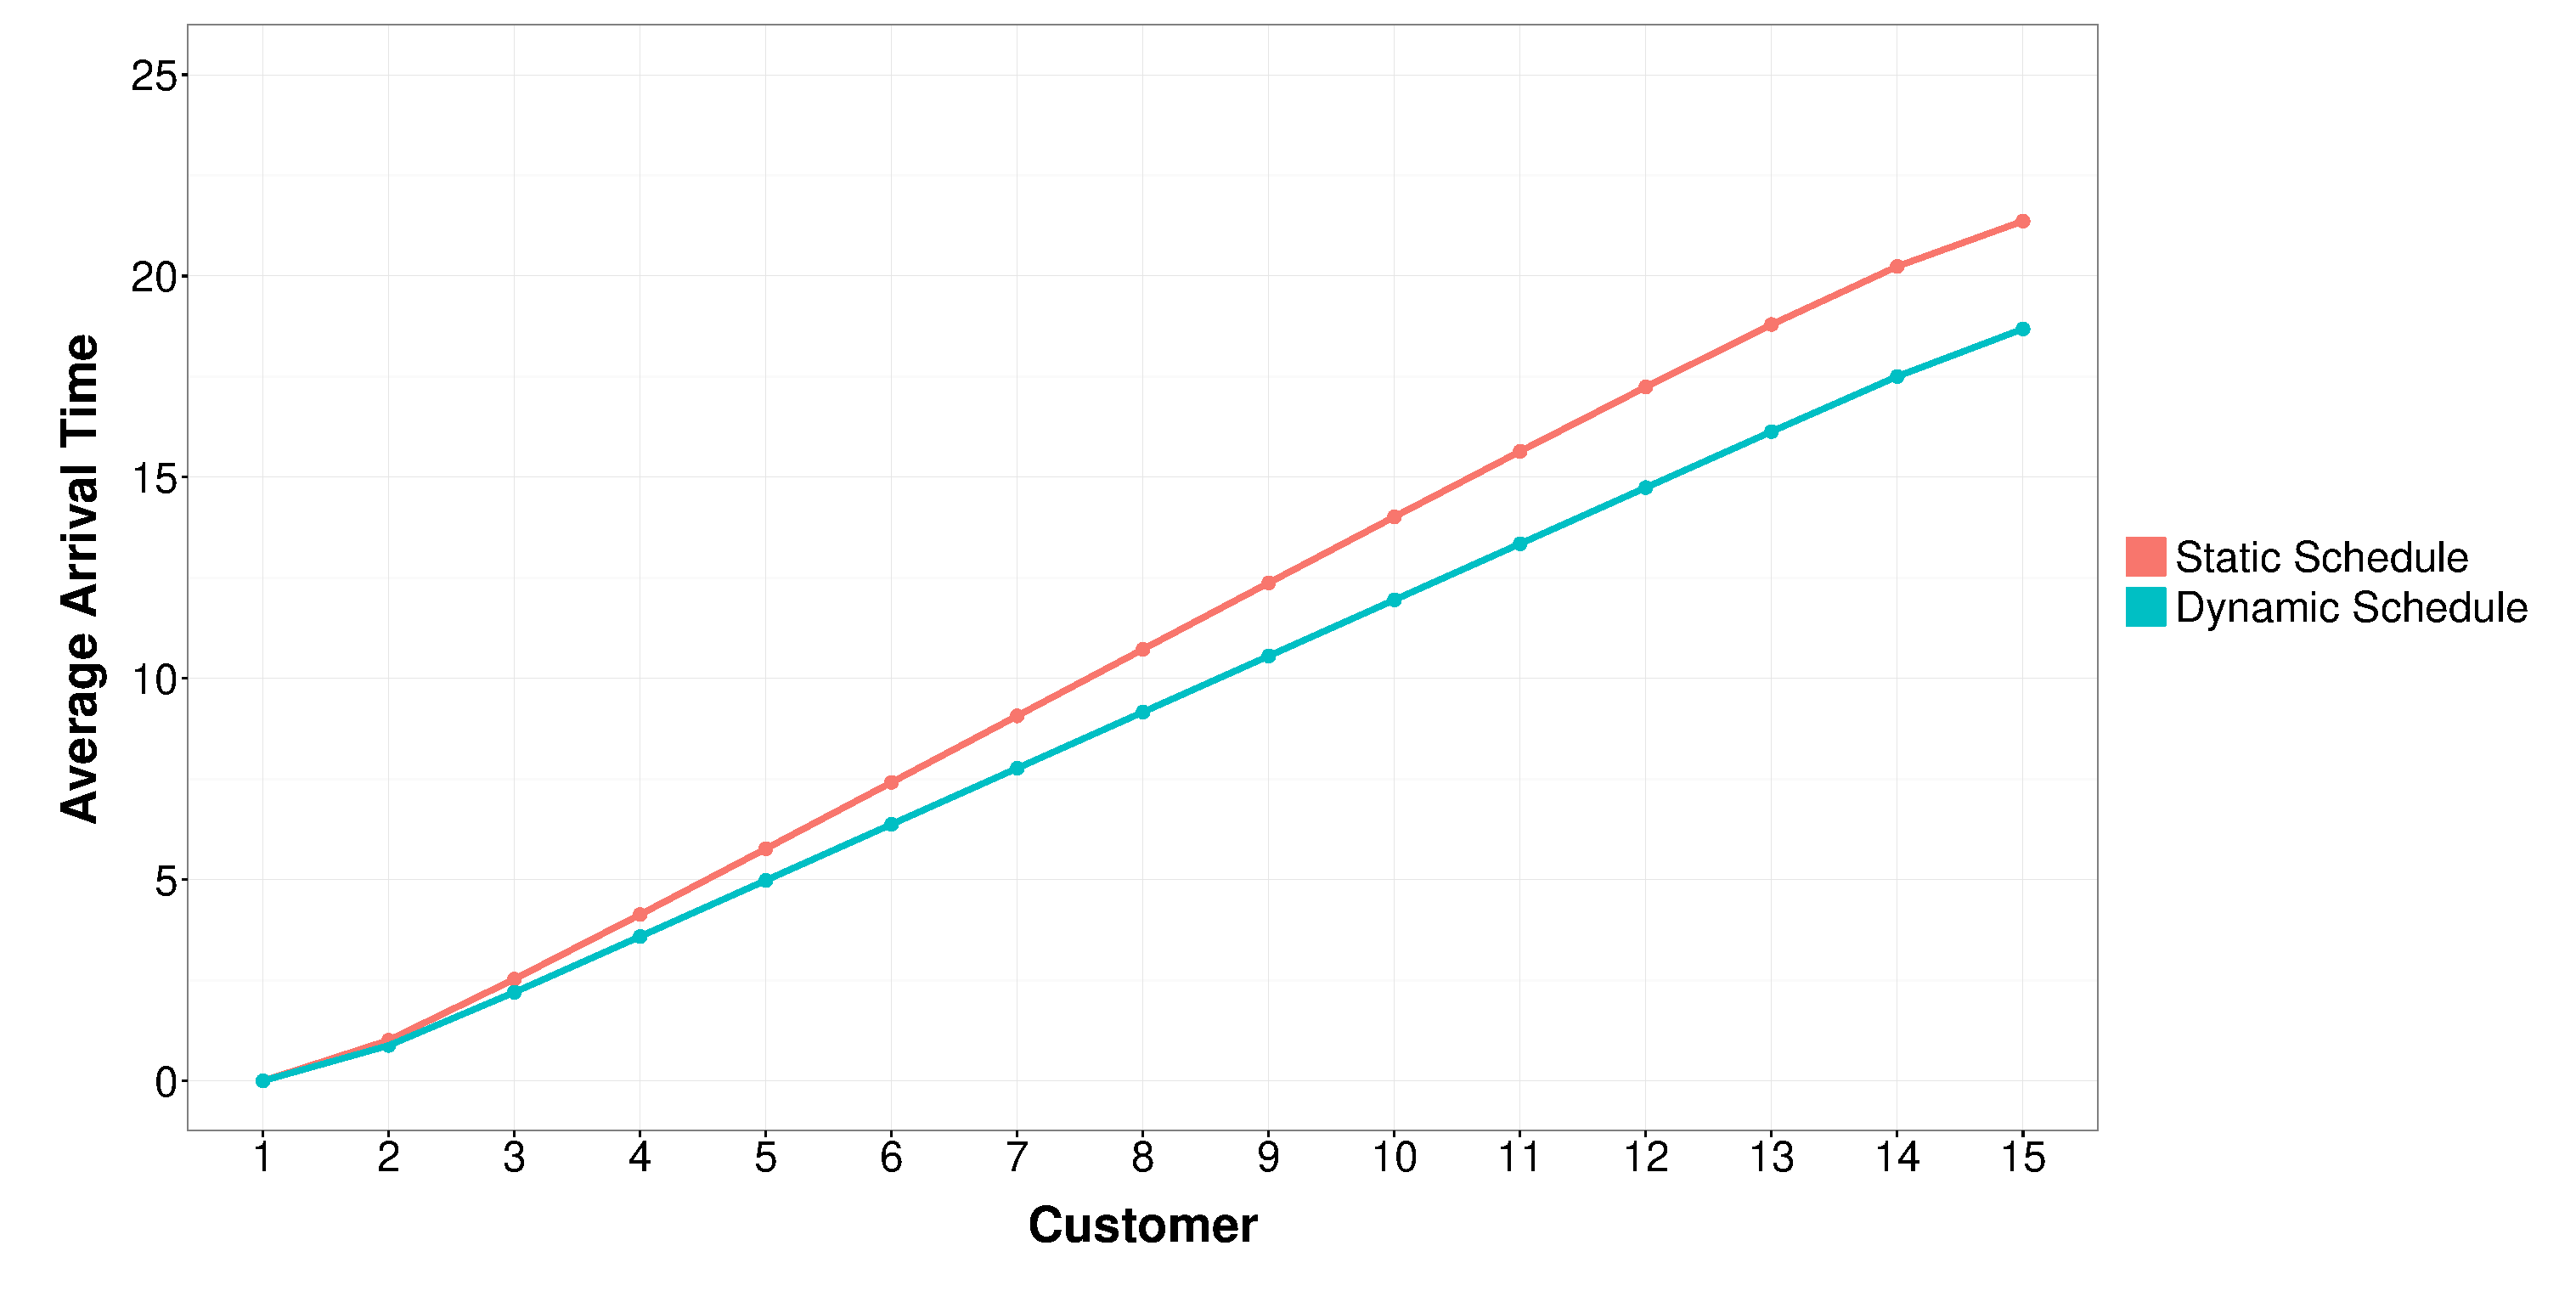
\includegraphics[width=\textwidth]{AT_Line.eps}
		\end{figure}
	\end{columns}
\end{frame}

\begin{frame}
	\begin{block}{Block Title}
		Lorem ipsum dolor sit amet, consectetur adipisicing elit, sed do eiusmod tempor incididunt ut labore et dolore magna aliqua.
	\end{block}
\end{frame}

\section{Section 2}

\begin{frame}
	Lorem ipsum dolor sit amet, consectetur adipisicing elit, sed do eiusmod tempor incididunt ut labore et dolore magna aliqua.
\end{frame}

\appendix

\section{Section 3}

\begin{frame}
	Lorem ipsum dolor sit amet, consectetur adipisicing elit, sed do eiusmod tempor incididunt ut labore et dolore magna aliqua.
\end{frame}

\end{document}









































